\documentclass{sig-alternate}
\usepackage{color}
\usepackage{algorithmic}
\usepackage{algorithm}

\let\oldbibliography\thebibliography
\renewcommand{\thebibliography}[1]{\oldbibliography{#1}
\vspace{0.3cm}
\setlength{\itemsep}{0pt}}


%%%% User-defined macros
\newcommand{\lam}{\lambda}
\newcommand{\mycomment}[1]{\textcolor{red}{#1}}
%%%%% Uncomment the following line and comment out the previous one
%%%%% to remove all comments
%%%%% NOTE: comments still occupy a line even if invisible;
%%%%% Don't write them as a separate paragraph
%\newcommand{\mycomment}[1]{}

\begin{document}

% --- Author Metadata here ---
%%% REMEMBER TO CHANGE THE SEMESTER AND YEAR
\conferenceinfo{UMM CSci Senior Seminar Conference, December 2013}{Morris, MN}

\title{Intrusion Detection with \\ Genetic Algorithms and Fuzzy Logic}

\numberofauthors{1}

\author{
% The command \alignauthor (no curly braces needed) should
% precede each author name, affiliation/snail-mail address and
% e-mail address. Additionally, tag each line of
% affiliation/address with \affaddr, and tag the
% e-mail address with \email.
\alignauthor
Emma Ireland\\
	\affaddr{Division of Science and Mathematics}\\
	\affaddr{University of Minnesota, Morris}\\
	\affaddr{Morris, Minnesota, USA 56267}\\
	\email{irela065@morris.umn.edu}
}

\maketitle
\begin{abstract}
Intrusion detection systems provide one way of detecting attacks on systems by monitoring network activities for malicious or abnormal behaviors. This paper describes two ways of training an intrusion detection system to recognize possible attacks on a system: genetic algorithms and fuzzy logic. I will describe an approach to using fuzzy genetic algorithms and compare those results with results obtained using a decision tree. I will then describe the results from using a traditional genetic algorithm and compare those with the winning entry of the KDD99 Classifier Learning Contest, as well as with the fuzzy genetic algorithm. These results show that the use of genetic algorithms and fuzzy logic in intrusion detection are effective ways of detecting attacks.
\end{abstract}

% A category with the (minimum) three required fields
%\category{}{Security and Privacy}{Intrusion Detection Systems}

%\terms{Security}

\keywords{Intrusion detection, genetic algorithms, fuzzy logic, KDD99, RLD09, computer security}

\section{Introduction}
The CSci computer lab at the University of Minnesota, Morris gets large numbers of login attempts that are attempts at intrusion. An attacker could be trying to gain root access to the system, which would then give them the ability to do things like delete files of other users and change user passwords. If the university had an intrusion detection system (IDS), it would be possible to classify those attempts into legitimate and illegitimate attempts to login. Then it would be possible to block IP addresses that are generating large numbers of attacks.

An attack on systems is a concern for many people, so it is important to have a way to detect and analyze these attacks. Intrusion detection systems provide one way of detecting attacks by monitoring network activities for malicious or abnormal behaviors and then producing reports, alerts, and actions~\cite{DBLP:journals/corr/abs-1204-1336}. There are various ways of training an IDS about possible threats. Two approaches that I will talk about in this paper are genetic algorithms and fuzzy logic.

In Section~\ref{sec:background} I will give some background on intrusion detection. I will describe the main types of networking attacks in Section~\ref{sec:typesAttacks}, and ways of detecting attacks in Section~\ref{sec:detectionMeth}. In Section~\ref{sec:dataSets} I will describe two data sets that are commonly used in intrusion detection. After that,  in Section~\ref{sec:PosNeg} I will describe the measures that are used in determining the accuracy of an IDS. I will then provide an overview on genetic algorithms in Section~\ref{sec:GA}. In Section~\ref{sec:fuzGenAlgImp} I will describe the use of a fuzzy genetic algorithm in an IDS, and in Section~\ref{sec:genAlgImp} I will describe the results of using a traditional genetic algorithm. Section~\ref{sec:conclusion} provides some conclusions about the use of genetic algorithms and fuzzy genetic algorithms in intrusion detection systems.




\section{Background}
\label{sec:background}

\subsection{Types of Networking Attacks}
\label{sec:typesAttacks}
There are four main types of networking attacks that this paper will address: \emph{denial of service attacks}, \emph{remote to user attacks}, \emph{user to root attacks}, and \emph{probe attacks}. Each attack that happens on a network can be placed into one of these categories.~\cite{DBLP:journals/corr/abs-1204-1336}

Denial of service (DoS) attacks happen when an attacker makes a machine inaccessible to a user by making it too busy to serve legitimate requests. For example, many systems lock out a user from an account after a certain number of failed login attempts. An attacker would be able to use this to prevent legitimate users from logging in, by intentionally failing to log in enough times to lock the account~\cite{DoSAttacks}. Remote to user, also known as remote to local (R2L) attacks happen when an attacker sends packets to a machine over the network in order to gain access to things a local user would have on the machine. An example is when an attacker tries to gain access to a machine by guessing possible usernames and passwords. User to root (U2R) attacks happen when an attacker starts out with access on the machine and then tries to gain root access to the system. If an attacker has access to an account on the machine, they could potentially run programs that take advantage of operating system weaknesses to gain root access. Probe attacks happen when an attacker examines a machine in order to collect information about weaknesses or vulnerabilities that in the future could be used to compromise the system. For example, the attacker could be trying to determine what version of a software is being run on that machine, and if that version has a known issue then that allows them to attempt to attack that.~\cite{DBLP:journals/corr/abs-1204-1336, typesOfAttacks}




\subsection{Detection Methodologies and Rules}
\label{sec:detectionMeth}
There are two different ways of detecting attacks: \emph{signature-based detection} and \emph{anomaly-based detection}. A signature is a pattern that corresponds to a known attack. Signature-based detection compares well-known patterns of attacks that are already known to the IDS against captured events in order to identify a possible attack. It is a simple and effective way to detect known attacks, but is ineffective against new kinds of unknown attacks. Signature-based detection is also called \emph{knowledge-based detection} or \emph{misuse detection}.~\cite{Liao201316}

Anomaly-based detection looks for patterns of activity that are rare and uncommon. It is harder to do than signature-based detection, but it can be an effective way to detect new, unknown attacks. Anomaly-based detection is also called \emph{behavior-based detection}.~\cite{DBLP:journals/corr/abs-1204-1336}

A commonly used approach for detecting intrusions is to use rules. Rules are represented by if-then statements in the following format: If (\emph{condition}) then (\emph{consequence}). The condition part of the rule is composed of one or more features, and the consequence of the rule says if it is an intrusion or not. For example: if (\emph{duration} = 1, and \emph{src\_bytes} = 0, and \emph{serror\_rate} = 50) then \emph{intrusion}.~\cite{Fries:2008:FAN:1388969.1389037}




\subsection{Data Sets}
\label{sec:dataSets}
Two different data sets are used in this paper to evaluate the performance of intrusion detection systems: KDD99 and RLD09. KDD99 is a benchmark data set that was generated by simulating a military network environment in 1999, and it has long been a standard data set for intrusion detection. The data was processed into five million records, where a record is a sequence of TCP packets, between which data flows to and from a source IP address to a target IP address. Each record in the data set is classified as either normal or attack activity. KDD99 uses 41 \emph{features}, which are properties of a record that are used to describe the activity and help to distinguish normal connections from attacks.~\cite{KDD99}

In the research discussed in Section~\ref{sec:fuzGenAlgImp}~\cite{6496342, 6559603}, eight of the 41 KDD99 features were used based on research done in~\cite{Fries:2008:FAN:1388969.1389037}. These eight features are:
\begin{enumerate}
\setlength{\itemsep}{1pt}
  \item duration: the length of the record in seconds.
  \item src\_bytes: the number of bytes sent from source to destination. Source is the user who may or may not be an attacker, and destination is the server being potentially attacked.
  \item num\_failed\_logins: the number of failed login attempts in this record.
  \item root\_shell: returns 1 if root shell is obtained, else it returns 0.
  \item num\_access\_files: the number of operations on access control files. Access control files specify which users are granted access to objects and what operations are allowed on the objects. An example would be (Alice, delete), which would give Alice permission to delete the file.~\cite{accessControl}
  \item srv\_count: the number of connections in other records.
  \item serror\_rate: the percentage of connections that have ``SYN" errors. When a client attempts to connect to a server, it first sends a SYN (synchronize) message to the server. The server then acknowledges the request by sending a SYN-ACK to the client. The connection is established when the client sends an ACK back to the server. A SYN error is a failure to get an ACK back.~\cite{TCP}
  \item same\_srv\_rate: the percentage of connections to the same service.
\end{enumerate}

The KDD99 data set is 14 years old, and newer attack types are not included in it because of its age. Because of this, the authors of~\cite{6496342, 6559603} created their own data set, RLD09, to use in their experiments. To create the data set, the authors captured network data from a university in Bangkok, Thailand. As well as normal network activity, RLD09 has 17 different types of attacks which can be classified as either denial of service attacks or probe attacks. RLD09 uses 12 features. For further information about the features, see~\cite{6496342}. In the research discussed in Section~\ref{sec:genAlgImp}, the authors of~\cite{DBLP:journals/corr/abs-1204-1336} used only the numerical features of KDD99 (34 out of 41).

In a machine learning experiment, a common technique is to divide the data set into two subsets, a \emph{training set} and a \emph{testing set}. The given algorithm is then trained on the training set to look for patterns. These patterns are then verified using the test set.~\cite{bc1_ecindm} This approach is used in~\cite{6496342, 6559603} and~\cite{DBLP:journals/corr/abs-1204-1336}.



\subsection{Determining the Accuracy of an Algorithm}
\label{sec:PosNeg}
Four measures are used to determine the accuracy of an algorithm. The \emph{false negative} (FN) rate is the percentage that attacks are misclassified from the total number of attack records. The \emph{false positive} (FP) rate is the percentage that normal records are classified as attacks from the total number of normal records. The \emph{true negative} (TN) rate is the percentage that normal records are classified correctly from the total number of normal records. The \emph{true positive} (TP) rate is the percentage that attacks are classified correctly from the total number of attack records.~\cite{6496342, bc1_ecindm}



\section{Genetic Algorithms}
\label{sec:GA}
Genetic algorithms (GAs) are a search technique used to find solutions to problems. Operations analogous to biological \emph{mutation}, \emph{selection}, and \emph{crossover} are used to evolve and improve solutions.

Possible solutions to problems can be represented in a variety of problem dependent ways, such as bit strings. For example, IDS rules can be represented as bit strings; see Section~\ref{sec:fuzzyRulesAndAlgorithm} for more information. First, a randomly generated population of potential solutions is created. Then mutation, crossover, and selection are applied to each generation until an acceptable solution is found or some time limit is exceeded.

Mutation is where random bits in an \emph{individual}, or possible solution, are randomly changed. Crossover is where two individuals swap sequences of bits to form two new individuals. For example, in an IDS mutation takes the bits of a rule and changes them to form a slightly different rule. Crossover takes two rules and creates new rules by swapping the bits of the old rules.

Selection is where individuals that have better \emph{fitness} are chosen to be parents. The fitness of an individual is specified by the \emph{fitness function}, which determines the quality of a particular individual. For example, in an IDS the fitness measures how well a rule classifies records as either attacks or normal activity. Selection combined with a fitness function directs the search towards an effective solution.~\cite{DBLP:journals/corr/abs-1204-6416}











\section{Using Fuzzy Genetic Algorithms}
\label{sec:fuzGenAlgImp}
The IDS used in~\cite{6496342, 6559603} is able to identify normal network activity as well as attacks using a fuzzy genetic algorithm. This kind of algorithm is able to learn to recognize new attacks.




\subsection{Fuzzy Logic Rules and Algorithm}
\label{sec:fuzzyRulesAndAlgorithm}
Attacks on systems do not always have a fixed pattern, so fuzzy logic is used to detect patterns that have a behavior that is between normal and unusual. Fuzzy logic rules are similar to the rules described in Section~\ref{sec:detectionMeth}, except that \emph{consequence} is a certainty factor. For example, if (\emph{duration} = 6) then (\emph{the degree of certainty of the record being an attack is 0.5}).

To find the degree of certainty of a record being an attack, a trapezoidal shape was used in~\cite{6496342, 6559603}; this is shown in Figure~\ref{fig:trapFigure}. The trapezoidal shape has four parameters: $a, b, c$, and $d$. Algorithm~\ref{alg:fuzAlg} calculates the certainty of a record being an attack.


\begin{figure}
\caption{Illustration of fuzzy rule used to find the degree of certainty of a record being an attack. Also see Algorithm~\ref{alg:fuzAlg}. This is used in~\cite{6496342, 6559603}.}
\centering
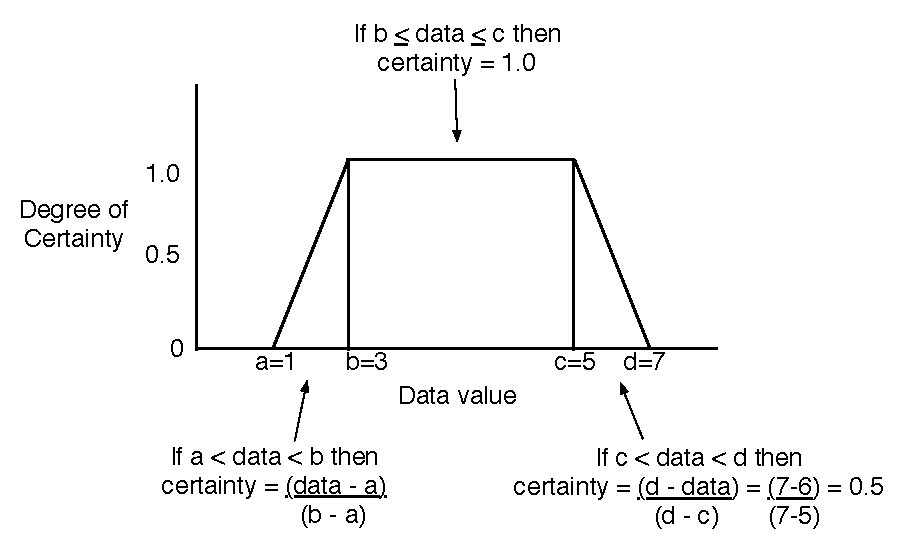
\psfig{file=trapFigExample.pdf, width=3.3in}
\label{fig:trapFigure}
\end{figure}

\begin{algorithm}[t]
\caption{Fuzzy Algorithm that is based on an algorithm used in~\cite{6496342, 6559603}, but a few corrections have been made. Also see Figure~\ref{fig:trapFigure}.}
\label{alg:fuzAlg}
\begin{algorithmic}
\IF{$b \leq \textrm{data} \leq c$}
  \STATE{certainty = 1.0}
\ELSIF{$a < \textrm{data} < b$}
  \STATE{
    certainty = $(\textrm{data}-a)/(b-a)$
  }
\ELSIF{$c < \textrm{data} < d$}
  \STATE{
    certainty = $(d-\textrm{data})/(d-c)$
  }
\ELSE \STATE{certainty = 0.0}
\ENDIF
\end{algorithmic}
\end{algorithm}

An example of using the fuzzy logic approach is: suppose that the feature is duration, and suppose it is 6 seconds, so then data = 6. Suppose that $a$ = 1, $b$ = 3, $c$ = 5, $d$~=~7. Because data (6) is between $c$ and $d$, then the degree of certainty of it being an attack is equal to

\begin{equation*}
\frac{d-\textrm{data}}{d-c} = \frac{7-6}{7-5} = 0.5.
\end{equation*}

The four parameters $a, b, c$, and $d$ are encoded into blocks of binary strings, where each block is a feature with values between 0 and 7. 
%See Figure~\ref{fig:fuzEncodingForFeature} for an example of a block. 
A rule has one block for each of 12 features followed at the end by a marker indicating the type of attack. An example of this is shown in Figure~\ref{fig:rule}. The authors of~\cite{6496342, 6559603} compute the degree of certainty for each of the 12 blocks, and if the sum of those is greater than a threshold, then it will be declared as an attack.

%\begin{figure}
%\centering
%\caption{Fuzzy encoding for a feature that is used in~\cite{6496342, 6559603}.}
%\vspace{0.20cm}
%\begin{tabular}{|cccc|} \hline
%010 & 011 & 100 & 101\\
%a=2 & b=3 & c=4 & d=5\\
%\hline\end{tabular}
%\label{fig:fuzEncodingForFeature}
%\end{figure}

\begin{figure*}
\centering
\caption{A rule with 12 blocks of features used in~\cite{6496342, 6559603}.}
\vspace{0.20cm}
\begin{tabular}{|cccc|c|cccc|c|} \hline
010 & 011 & 100 & 101   & ...... & 010 & 011 & 101 & 111   & DoS\\
a=2 & b=3 & c=4 & d=5   & ...... & a=2 & b=3 & c=5 & d=7   &\\ 
    &     & Block 1&    &        &     & Block 12& &       & Type\\
\hline\end{tabular}
\label{fig:rule}
\end{figure*}




\subsection{Algorithm Overview}
The algorithm in~\cite{6496342, 6559603} first randomly generates rules. Then the rules are improved in the training phase, which can be seen in Algorithm~\ref{alg:fuzGenAlg}, which describes the fuzzy genetic algorithm that is used. One record (either an attack or normal activity) is passed into a rule. Each feature in a record is matched to one block of the rule. The parameters of each block measure the degree of certainty of an attack using the trapezoidal fuzzy rule shape. The sum of the degrees of certainty from each block are then compared with a threshold to determine if the record represents an attack or normal behavior.

\begin{algorithm}[t]
\caption{Fuzzy GA that is based on an algorithm used in~\cite{6496342, 6559603}, but a few corrections have been made.}
\label{alg:fuzGenAlg}
\begin{algorithmic}
\FOR{each rule}

  \FOR{each record}
    \FOR{each feature}
      \STATE{certainty = fuzzy(); // Algorithm~\ref{alg:fuzAlg}}
      \STATE{total = total + certainty;}
    \ENDFOR
    
    \IF{total > threshold} 
      \STATE{class is attack;}
      \ELSE \STATE{class is normal;}
    \ENDIF
  \ENDFOR
  
  \STATE{compare the predicted result with actual result}
  \STATE{find $A$, $B$, $\alpha$, and $\beta$}
  \STATE{// $A$ is the total number of attack records. $B$ is the total number of normal records. $\alpha$ is the total number of attack records correctly identified as attack. $\beta$ is the total number of normal records incorrectly classified as attack.}
\ENDFOR
\STATE{calculate fitness}
\STATE{//create next generation}
\STATE{preserve\_best()}
\STATE{crossover()}
\STATE{mutation()}
\end{algorithmic}
\end{algorithm}


The fitness function to be maximized in Algorithm~\ref{alg:fuzGenAlg} is:
\begin{equation*}
\textrm{fitness function} = \frac{\alpha}{A} - \frac{\beta}{B}
\end{equation*}
where $A$ is the total number of attack records, $B$ is the total number of normal records, $\alpha$ is the total number of attack records correctly identified as attack, and $\beta$ is the total number of normal records incorrectly classified as attack.

A population size of 10 was used for each generation. The two best individuals from the present generation are preserved for the next generation. The other individuals in the new generation come from mutation and crossover.



\newpage




\subsection{Experimental Design and Results}
\label{sec:experimentalDesignResults}
A variety of experiments were run in~\cite{6496342, 6559603}. Two experiments used just RLD09, and three experiments used KDD99 and RLD09 together.

\subsubsection{Experiments using Only RLD09}
The experiments using only RLD09 that~\cite{6496342} performed used a total of 16,000 records of normal activity and 10,500 records of attack activity. Of the attack records, 4,000 were denial of service attacks and 6,500 were probe attacks.

In the first experiment, the fuzzy genetic algorithm was used to create separate denial of service and probe detection rules. Both of the denial of service and probe rules were then used together in the testing process to identify attacks from the testing data set; this is shown in Algorithm~\ref{alg:identifyAttacks}. 10,000 records were used for the training set and all 26,500 records were used for the testing set. (The authors of~\cite{6496342} really should not have reused the training data in the testing set because it inflates their results.)

\begin{algorithm}[t]
\caption{This algorithm was used to identify attacks and normal activity in~\cite{6496342}.}
\label{alg:identifyAttacks}
\begin{algorithmic}
\IF{dos\_rule = yes or probe\_rule = yes} 
	\STATE{This record is an attack;}
\ELSE \STATE{This record is normal;}
\ENDIF
\end{algorithmic}
\end{algorithm}

To evaluate the accuracy of the fuzzy genetic algorithm, detection rate (DR) was used. Detection rate is defined in~\cite{6496342, 6559603} as the percentage of normal and attack activity correctly classified from the total number of data records. The detection rate of DoS attacks in training was 91.64\% and the detection rate of probe attacks in training was 94.79\%. The detection rate of the testing data set increased to 97.92\%. Results from this experiment are in Table~\ref{tab:fuzGenExp1}.

\begin{table*}
\center
\caption{Results from Experiment 1, using only RLD09~\cite{6496342}.}
\vspace{0.20cm}
\begin{tabular}{ccccccc}
 & Attack & Normal & Total Records & FP (\%) & FN (\%) & DR (\%)\\
DoS Training & 1499 & 8501 & 10000 & 1.46 & 47.50 & 91.64\\
Probe Training & 2496 & 7504 & 10000 & 1.83 & 15.38 & 94.79\\
Testing & 10500 & 16000 & 26500 & 1.13 & 4.10 & 97.92\\
\end{tabular}
\label{tab:fuzGenExp1}
\center
\end{table*}

In the second experiment,~\cite{6496342} pulled some types of attacks out of the training set and kept them for unknown data testing. This was to test that the fuzzy genetic algorithm could detect unknown attacks. In this experiment, seven tests were run. For each test case there were 13 attack types plus normal activity that were in the training data set. Three attack types were used for the unknown testing data set. For example, test case 1 used the training data set that does not have Advance Port Scan, Ack Scan, and Xmas Tree, which are all probe attacks. These three attacks were then used for the testing data set. Table~\ref{tab:fuzGenExp2} shows the results from the fuzzy genetic algorithm and a decision tree algorithm, which is another common algorithm for classification problems. For further information on decision trees, see~\cite{decisionTree}, and for further information on the types of denial of service and probe attacks, see~\cite{typesOfAttacks}. When compared with the decision tree algorithm, the fuzzy genetic algorithm has a higher detection rate in all cases except 5 and 7, however, no information on statistical significance was given.


\begin{table}
\caption{Unknown attack experiment, using only the RLD09 data set~\cite{6496342}.}
\vspace{0.20cm}
\begin{tabular}{llll}
Test & Unknown & Decision & Fuzzy GA\\
Case & Attacks & Tree DR (\%)  & DR (\%)\\ \hline

1 & Adv Port Scan (Probe) & Avg = & Avg =\\
  & Ack Scan (Probe)		  & 98.33 & 100\\
  & Xmas Tree (Probe)		  &		  &\\ \hline

2 & HTTP Flood (DoS) & Avg = & Avg =\\
  & IP Scan (Probe)		& 88.4 & 95.30\\
  & Null Scan (Probe)	&		  &\\ \hline

3 & Smurf (DoS) & Avg = & Avg =\\
  & Port Scan (Probe)		& 97.65 & 99.15\\
  & Connect Scan (Probe)	&		  &\\ \hline

4 & UDP Flood (DoS) & Avg = & Avg =\\
  & Host Scan (Probe) & 46.65 & 99.80\\
  & UDP Scan (Probe)  &       &\\ \hline

5 & Jping (DoS)    & Avg =          & Avg =\\
  & Syn Scan (Probe) & 99.70 & 98.75\\
  & Fin Scan (Probe) &                &\\ \hline

6 & UDP Flood (DoS) & Avg = & Avg =\\
  & RCP Scan (Probe)  & 70.35 & 98.15\\
  & Fin Scan (Probe)  &       &\\ \hline

7 & HTTP Flood (DoS) & Avg =          & Avg =\\
  & RCP Scan (Probe)  & 99.94 & 97.50\\
  & Fin Scan (Probe) &                &\\
\hline\end{tabular}
\label{tab:fuzGenExp2}
\end{table}




\subsubsection{Experiments using Both RLD09 and KDD99}
The authors of~\cite{6559603} also ran experiments that used both the RLD09 data set and the KDD99 data set in order to compare how the fuzzy genetic algorithm would perform on both. They used a subset of the KDD99 data set for both the training data set and testing data set.

The first experiment used the fuzzy genetic algorithm to classify normal activity and attacks from both data sets. The authors of~\cite{6559603} first trained and tested the fuzzy genetic algorithm (Algorithm~\ref{alg:fuzGenAlg}) with the KDD99 data set. There were 6 different types of denial of service attacks and 4 different types of probe attacks. The detection rate of the KDD99 data set was 98.72\%. Then 26,500 records of the RLD09 data set were used as the training set. The detection rate was 97.97\%. The results of this experiment are shown in Table~\ref{tab:bothSetsResults}.

\begin{table}
\caption{KDD99 and RLD09 results from the first experiment in~\cite{6559603}.}
\vspace{0.20cm}
\begin{tabular}{llllll}
Data set & Attack & Normal & FP(\%) & FN(\%) & DR(\%)\\ \hline
KDD99 & 160,117 & 39,337 & 0.13 & 1.55 & 98.72\\
RLD09 & 10,500 & 16,000 & 1.14 & 3.39 & 97.97\\
\end{tabular}
\label{tab:bothSetsResults}
\end{table}

The next experiment used the fuzzy genetic algorithm to classify types of attacks in the KDD99 data set. They used the KDD99 training set, with 158,597 records of denial of service attacks and 1,500 records of probe attacks. Ten tests were run, and Table~\ref{tab:kddAttacks} shows the accuracy of detecting some of the cases. The results showed that the detection rate of eight out of ten cases were greater than 93\%. There were only two cases that had low detection rates, one of which is case 1 in Table~\ref{tab:kddAttacks}. The two low detection rates were 16.56\% and 15.58\%, both of which were denial of service attacks.

\begin{table}
\caption{Results for KDD99 with Certain Attacks. 10 tests were run in total, 5 are shown here.~\cite{6559603}}
\vspace{0.20cm}
\begin{tabular}{cccccc}
Test & Attack & Type & FP(\%) & FN(\%) & DR(\%)\\ \hline
1 & Back & DoS & 85.33 & 0.00 & 16.56\\
2 & Smurf & DoS & 0.76 & 0.10 & 99.73\\
3 & Neptune & DoS & 0.15 & 0.34 & 99.75\\
4 & Portsweep & Probe & 6.40 & 0.00 & 93.66\\
5 & Satan & Probe & 0.74 & 3.75 & 99.22\\
\end{tabular}
\label{tab:kddAttacks}
\end{table}

The final experiment that was run used only the RLD09 data set with the fuzzy genetic algorithm to classify types of attacks. 17 tests were run, and Table~\ref{tab:rldAttacks} shows the accuracy of detecting some of the cases. The results showed that the detection rate of 15 out of 17 cases were greater than 97\%. Again, there were only two test cases that had low detection rates, cases 3 and 5 in Table~\ref{tab:rldAttacks}. The two low detection rates were 89.59\% (denial of service), and 86.89\% (probe).

\begin{table}
\caption{Results for RLD09 with Certain Attacks. 17 tests were run in total, 6 are shown here.~\cite{6559603}}
\vspace{0.20cm}
\begin{tabular}{cccccc}
Test & Attack & Type & FP(\%) & FN(\%) & DR(\%)\\ \hline
1 & HTTP Flood & DoS & 0.36 & 3.5 & 99.46\\
2 & Smurf & DoS & 0.02 & 0 & 99.98\\
3 & UDP Flood & DoS & 11.06 & 0 & 89.59\\
4 & Fin Scan & Probe & 2.58 & 0 & 97.50\\
5 & IP Scan & Probe & 13.01 & 16.4 & 86.89\\
6 & Syn Scan & Probe & 0.65 & 4.2 & 99.24\\
\end{tabular}
\label{tab:rldAttacks}
\end{table}












\section{Using Genetic Algorithms}
\label{sec:genAlgImp}

The authors of~\cite{DBLP:journals/corr/abs-1204-1336} used a genetic algorithm to develop an IDS. They didn't explain their research that well and left a lot of things out, so I will just be describing their results.

The KDD99 data set was used in the experiments. Standard subsets of the set were used for training and testing. The training set had a total of 494,021 records, 396,741 of which were attacks. The test set had a total of 311,029 records, 250,436 of which were attacks. Table~\ref{tab:numberOfRecords} shows the distribution of each type of attack, as well as normal activity, that were in the training and test sets.

\begin{table}
\center
\caption{Training and testing records used in~\cite{DBLP:journals/corr/abs-1204-1336}.}
\vspace{0.20cm}
\begin{tabular}{lll}
  & Training & Testing \\ 
Normal & 97,280 & 60,593\\ \hline
DoS	   & 391,458 & 229,853\\
R2L    & 1,124   & 16,189\\
U2R    & 52      & 228\\
Probe  & 4,107  & 4,166\\ \hline
Total Attacks & 396,741 & 250,436 \\
Total Records  & 494,021 & 311,029\\
\end{tabular}
\center
\label{tab:numberOfRecords}
\end{table}



The results from running the genetic algorithm are shown in Table~\ref{tab:genAlgResults}. Detection rate is defined in~\cite{DBLP:journals/corr/abs-1204-1336} as the ratio between the number of correctly detected intrusions and the total number of intrusions. Denial of service attacks had the highest detection rate at 99.4\%. A high detection rate on denial of service attacks isn't surprising because there were a lot of denial of service records used compared with the other types of attacks. The accuracy of the genetic algorithm is shown in Table~\ref{tab:genAlgResults2}. The true negative rate was 69.5\%. The false positive rate was 30.5\%. The false negative rate was 5\%. The true positive rate was 94.9\%.

\begin{table*}
\center
\caption{Results for GA Experiment in~\cite{DBLP:journals/corr/abs-1204-1336}.}
\vspace{0.20cm}
\begin{tabular}{l|cccccc}
& & & Predicted & & & \\
Actual & Normal & Probe & DoS & U2R & R2L & \% Correct \\ \hline
Normal & 42138 & 1421 & 15835 & 486 & 713 & 69.5\\
Probe & 398 & 2963 & 654 & 2 & 149 & 71.1   \\
Dos & 921 & 432 & 228489 & 1 & 10 & 99.4\\
U2R & 146 & 21 & 8 & 43 & 10 & 18.9\\
R2L & 11191 & 578 & 3398 & 141 & 881 & 5.4\\
& &&&&& \\
\% Correct &  76.9 & 54.7 & 92.0 & 6.4 & 50.0 & \\
\end{tabular}
\center
\label{tab:genAlgResults}
\end{table*}



\begin{table}
\center
\caption{Accuracy of the GA in~\cite{DBLP:journals/corr/abs-1204-1336}.}
\vspace{0.20cm}
Predicted
\begin{tabular}{l|ll}
Actual & Normal & Attack \\ \hline
Normal & TN: 42,138. 69.5\% & FP: 18,455. 30.5\% \\
Attack & FN: 12,528. 5\% & TP: 237,908. 94.9\%  \\
\end{tabular}
\center
\label{tab:genAlgResults2}
\end{table}


The authors of~\cite{DBLP:journals/corr/abs-1204-1336} compared their results (Table~\ref{tab:genAlgResults}) with the winning entry of the KDD99 Classifier Learning Contest~\cite{KDD99Contest}, which can be seen in Table~\ref{tab:winningEntry}. The winning entry used a decision tree algorithm. The winning entry had a higher detection rate for normal activity, probe attacks, and remote to user attacks. The authors of~\cite{DBLP:journals/corr/abs-1204-1336} found that they had a better detection rate for denial of service and user to root attacks than the winning entry. For the winning entry, the detection rate of denial of service was 97.1\%, and for user to root it was 13.2\%. In~\cite{DBLP:journals/corr/abs-1204-1336} the detection rate of denial of service was 99.4\% and for user to root it was 18.9\%. The authors of~\cite{DBLP:journals/corr/abs-1204-1336} provide no information about the statistical significance of these improvements.

\begin{table*}
\center
\caption{Results for the Winning Entry of the KDD99 Classifier Learning Contest.}
\vspace{0.20cm}
\begin{tabular}{l|cccccc}
& & & Predicted & & &\\
Actual & Normal & Probe & DoS & U2R & R2L & \% Correct \\ \hline
Normal &  60262 & 243 & 78 & 4 & 6 & 99.5\\
Probe &  511 & 3471 & 184 & 0 & 0 & 83.3 \\
Dos &  5299 & 1328 & 223226 & 0 & 0 & 97.1\\
U2R &  168 & 20 & 0 & 30 & 10 & 13.2\\
R2L &  14527 & 294 & 0 & 8 & 1360 & 8.4\\
& &&&&& \\
\% Correct &  74.6 & 64.8 & 99.9 & 71.4 & 98.8 &\\
\end{tabular}
\center
\label{tab:winningEntry}
\end{table*}

The detection rate (as defined in Section~\ref{sec:experimentalDesignResults} and~\cite{6559603}) of the traditional genetic algorithm in~\cite{DBLP:journals/corr/abs-1204-1336} was 90\% (see Tables~\ref{tab:genAlgResults2} and~\ref{tab:numberOfRecords}). This means that it correctly classified 90\% of the test records. The detection rate of the fuzzy genetic algorithm in~\cite{6559603} was 99\% (see Table~\ref{tab:bothSetsResults}). The fuzzy genetic algorithm in~\cite{6559603} is not the same as the traditional genetic algorithm in~\cite{DBLP:journals/corr/abs-1204-1336} with fuzzy logic added to it, but it can be said that the system in~\cite{6559603} is better than~\cite{DBLP:journals/corr/abs-1204-1336} however it was built.

\section{Conclusions}
\label{sec:conclusion}
The fuzzy genetic algorithm that was used in~\cite{6496342, 6559603} had a higher detection rate than a decision tree algorithm in most cases, and it was good at detecting unknown attacks. It had a higher detection rate than the traditional genetic algorithm that was used in~\cite{DBLP:journals/corr/abs-1204-1336}. The genetic algorithm in~\cite{DBLP:journals/corr/abs-1204-1336} had a high detection rate for denial of service attacks. When compared with the winning entry of the KDD99 Classifier Learning Contest, it was shown to have a better detection rate for both denial of service and user to root attacks. This paper showed that the use of genetic algorithms and fuzzy genetic algorithms in intrusion detection are effective ways of detecting attacks.


%\section{Acknowledgments}




% The following two commands are all you need in the
% initial runs of your .tex file to
% produce the bibliography for the citations in your paper.
\bibliographystyle{abbrv}
% sample_paper.bib is the name of the BibTex file containing the
% bibliography entries. Note that you *don't* include the .bib ending here.
\bibliography{annotated_bibliography}  
% You must have a proper ".bib" file
%  and remember to run:
% latex bibtex latex latex
% to resolve all references

\end{document}
